\chapter{Probabilité conditionnelle}

\section{Calcul à l'aide d'un tableau croisé}

\subsection{Tableau d'effectifs et de fréquences}

Dans une étude statistique portant sur deux caractères, on organise souvent les données dans un tableau croisé à double entrée (ou tableau d'effectifs).

\begin{ex}
	On a interrogé $200$ personnes sur leur pratique sportive. Les résultats sont consignés ci-dessous :

	\begin{center}
		\def\arraystretch{1.5}
		\begin{tabular}{|l|c|c|c|} \hline
			                                & \textbf{Sportif $\pa{S}$} & \textbf{Non-sportif $\pa{\bar{S}}$} & \textbf{Total} \\ \hline
			\textbf{Jeunes $\pa{J}$}        & $45$                      & $15$                                & \textbf{60}    \\ \hline
			\textbf{Adultes $\pa{\bar{J}}$} & $80$                      & $60$                                & \textbf{140}   \\ \hline
			\textbf{Total}                  & \textbf{125}              & \textbf{75}                         & \textbf{200}   \\ \hline
		\end{tabular}
	\end{center}

	\begin{itemize}
		\item \textbf{Effectif total :} $\text{Card}(\Omega) = 200$ personnes.
		\item \textbf{Effectif de l'intersection :} $\text{Card}(J \cap S) = 45$ personnes sont à la fois \og{}Jeunes\fg{} \textbf{et} \og{}Sportifs\fg{}.
		\item \textbf{Effectifs marginaux :} $\text{Card}(J) = 60$ personnes sont jeunes ; $\text{Card}(S) = 125$ personnes sont sportives.
	\end{itemize}
\end{ex}

\begin{defin}[Fréquences marginales et conditionnelles]
	Soit un tableau d'effectifs croisant deux caractères :
	\begin{itemize}
		\item Une \textbf{fréquence marginale} est la fréquence d'un caractère calculée par rapport à l'effectif total.

		      Elle se lit dans les marges du tableau.
		\item Une \textbf{fréquence conditionnelle} est la fréquence d'un caractère calculée en se restreignant à une ligne ou une colonne précise (sous-population).
	\end{itemize}
\end{defin}

\begin{methode}[Calculer des fréquences conditionnelles]
	En reprenant l'exemple précédent :
	\begin{enumerate}
		\item La fréquence marginale des jeunes est :
		      \[
			      f_J = \dfrac{60}{200} = 0,30 = 30\%
		      \]
		\item La fréquence conditionnelle des sportifs parmi les jeunes se calcule en se limitant à la ligne \og{}Jeunes\fg{} :
		      \[
			      f_{\text{sportif sachant jeune}} = \dfrac{45}{60} = 0,75 = 75\%
		      \]
		\item La fréquence conditionnelle des jeunes parmi les sportifs se calcule en se limitant à la colonne \og{}Sportif\fg{} :
		      \[
			      f_{\text{jeune sachant sportif}} = \dfrac{45}{125} = 0,36 = 36\%
		      \]
	\end{enumerate}
\end{methode}

\section{Probabilités conditionnelles}

\subsection{Définition et calculs}

\begin{defin}[Probabilité conditionnelle]
	Soit $A$ un événement de probabilité non nulle.

	On appelle \textbf{probabilité conditionnelle} de $B$ sachant $A$, la probabilité que l'événement $B$ se réalise sachant que l'événement $A$ est réalisé.

	Elle se note $P_A(B)$.
\end{defin}

\begin{ex}
	On considère l'expérience aléatoire qui consiste à \textbf{choisir une personne au hasard} parmi les $200$ personnes interrogées dans l'étude précédente.

	L'univers $\Omega$ est l'ensemble de ces $200$ personnes ($\text{Card}(\Omega) = 200$).

	On définit les événements suivants :

	\begin{itemize}
		\item $J$ : \og{}La personne choisie est jeune\fg{} ;
		\item $S$ : \og{}La personne choisie est sportive\fg{}.
	\end{itemize}

	On a donc :

	\begin{itemize}
		\item $P(S)$ est la probabilité qu'une personne prise au hasard dans \textbf{toute la population} soit sportive ($125$ personnes sur $200$).
		\item $P_J(S)$ est la probabilité qu'une personne soit sportive \textbf{sachant qu'elle fait partie des jeunes}.

		      On ne regarde plus tout le monde, on se focalise uniquement sur le groupe des jeunes ($45$ sportifs sur les $60$ jeunes).
	\end{itemize}
\end{ex}

\begin{prop}[Calculs de probabilités conditionnelles]
	Pour tout événement $A$ tel que $P(A) \neq 0$ :
	\begin{itemize}
		\item \textbf{Formule générale :}
		      \[
			      P_A(B) = \dfrac{P(A \cap B)}{P(A)}
		      \]
		\item \textbf{Lien avec les effectifs (équiprobabilité) :}
		      \[
			      P_A(B) = \dfrac{\text{Card}(A \cap B)}{\text{Card}(A)}
		      \]
	\end{itemize}
\end{prop}

\begin{methode}[Calculer une probabilité conditionnelle à partir d'un tableau]
	Un laboratoire pharmaceutique réalise une étude sur 800 patients :

	\begin{center}
		\def\arraystretch{1.5}
		\begin{tabular}{|l|c|c|c|} \hline
			                                  & \textbf{Médicament A} & \textbf{Médicament B} & \textbf{Total} \\ \hline
			\textbf{Guéri $\pa{G}$}           & $383$                 & $291$                 & $674$          \\ \hline
			\textbf{Non guéri $\pa{\bar{G}}$} & $72$                  & $54$                  & $126$          \\ \hline
			\textbf{Total}                    & $455$                 & $345$                 & $800$          \\ \hline
		\end{tabular}
	\end{center}

	On choisit un patient au hasard.
	\begin{enumerate}
		\item Probabilité que le patient soit guéri : $P(G) = \dfrac{674}{800} = 0,8425$.
		\item Probabilité que le patient ait pris le médicament A sachant qu'il est guéri :
		      \[
			      P_G(A) = \dfrac{\text{Card}(A \cap G)}{\text{Card}(G)} = \dfrac{383}{674} \approx 0,568
		      \]
	\end{enumerate}
\end{methode}

\section{Représentation par un arbre pondéré}

\subsection{Construction et règles de lecture}

Un arbre pondéré permet de modéliser une succession d'épreuves.

\begin{center}
	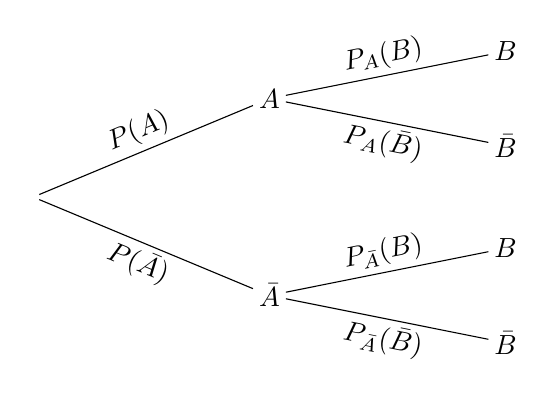
\begin{tikzpicture}[
			grow=right,
			level 1/.style={level distance=3cm, sibling distance=2.5cm},
			level 2/.style={level distance=3cm, sibling distance=1.2cm},
			every node/.style={inner sep=2pt}
		]
		\node {}
		child { node { $\bar{A}$ }
				child { node { $\bar{B}$ } edge from parent node[sloped, below] { $P_{\bar{A}}(\bar{B})$ } }
				child { node { $B$ } edge from parent node[sloped, above] { $P_{\bar{A}}(B)$ } }
				edge from parent node[sloped, below] { $P(\bar{A})$ }
			}
		child { node { $A$ }
				child { node { $\bar{B}$ } edge from parent node[sloped, below] { $P_A(\bar{B})$ } }
				child { node { $B$ } edge from parent node[sloped, above] { $P_A(B)$ } }
				edge from parent node[sloped, above] { $P(A)$ }
			};
	\end{tikzpicture}
\end{center}

\begin{ex}
	On choisit un élève au hasard dans un lycée et on note :
	\begin{itemize}
		\item $F$ : \og{}L'élève est une fille\fg{}
		\item $L$ : \og{}L'élève a les cheveux longs\fg{}
	\end{itemize}

	On suppose que le lycée compte $45\%$ de filles.

	Dans ce lycée :
	\begin{itemize}
		\item $60\%$ des filles ont les cheveux longs ($P_F(L) = 0{,}6$) ;
		\item $20\%$ des garçons ont les cheveux longs ($P_{\bar{F}}(L) = 0{,}2$).
	\end{itemize}

	\begin{center}
		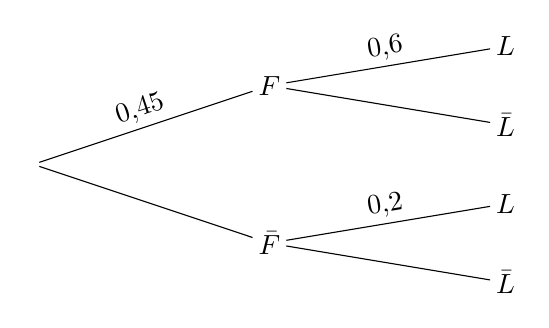
\begin{tikzpicture}[
				grow=right,
				level 1/.style={level distance=3cm, sibling distance=2cm},
				level 2/.style={level distance=3cm, sibling distance=1cm},
				every node/.style={inner sep=2pt}
			]
			\node {}
			child { node { $\bar{F}$ }
					child { node { $\bar{L}$ } edge from parent node[sloped, below] {  } }
					child { node { $L$ } edge from parent node[sloped, above] { $0{,}2$ } }
					edge from parent node[sloped, below] {  }
				}
			child { node { $F$ }
					child { node { $\bar{L}$ } edge from parent node[sloped, below] {  } }
					child { node { $L$ } edge from parent node[sloped, above] { $0{,}6$ } }
					edge from parent node[sloped, above] { $0{,}45$ }
				};
		\end{tikzpicture}
	\end{center}
\end{ex}

\begin{prop}[Règles des n\oe{}uds]
	\nline
	\begin{wrapstuff}[r]
		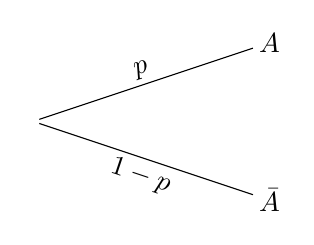
\begin{tikzpicture}[ grow=right, level 1/.style={level distance=3cm, sibling distance=2cm}, every node/.style={inner sep=2pt} ]
			\node {}
			child { node { $\bar{A}$ } edge from parent node[sloped, below] { $1-p$ } }
			child { node { $A$ } edge from parent node[sloped, above] { $p$ } };
		\end{tikzpicture}
	\end{wrapstuff}

	La somme des probabilités des branches issues d'un même n\oe{}ud est égale à 1.
	\[
		P(A) + P(\bar{A}) = 1 \quad \text{et} \quad P_A(B) + P_A(\bar{B}) = 1
	\]

	\phantom{x}

	\phantom{x}
\end{prop}

\begin{prop}[Probabilité d'une intersection]
	\nline
	\begin{wrapstuff}[r]
		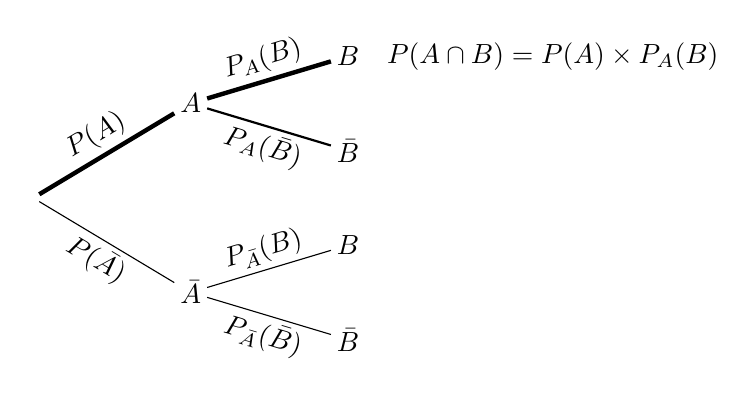
\begin{tikzpicture}[
				grow=right,
				level 1/.style={level distance=2cm, sibling distance=2.4cm},
				level 2/.style={level distance=2cm, sibling distance=1.2cm},
				every node/.style={inner sep=2pt}
			]
			\node {}
			child { node { $\bar{A}$ }
					child { node { $\bar{B}$ } edge from parent node[sloped, below] { $P_{\bar{A}}(\bar{B})$ } }
					child { node { $B$ } edge from parent node[sloped, above] { $P_{\bar{A}}(B)$ } }
					edge from parent node[sloped, below] { $P(\bar{A})$ }
				}
			child { node { $A$ }
					child { node { $\bar{B}$ } edge from parent[thick] node[sloped, below] { $P_A(\bar{B})$ } }
					child { node { $B$ }
							node[right=0.3cm] {$\rarr\  P(A \cap B) = P(A) \times P_A(B)$}
							edge from parent[ultra thick] node[sloped, above] { $P_A(B)$ }
						}
					edge from parent[ultra thick] node[sloped, above] { $P(A)$ }
				};
		\end{tikzpicture}
	\end{wrapstuff}
	La probabilité de l'événement situé au bout d'un chemin est le produit des probabilités rencontrées sur ce chemin.
	\[
		P(A \cap B) = P(A) \times P_A(B)
	\]

	\phantom{x}

	\phantom{x}

	\phantom{x}

	\phantom{x}
\end{prop}

\begin{ex}[Calcul d'une intersection et règle des n\oe{}uds]
	On reprend l'exemple de la répartition des élèves selon le sexe et la longueur des cheveux :
	\begin{center}
		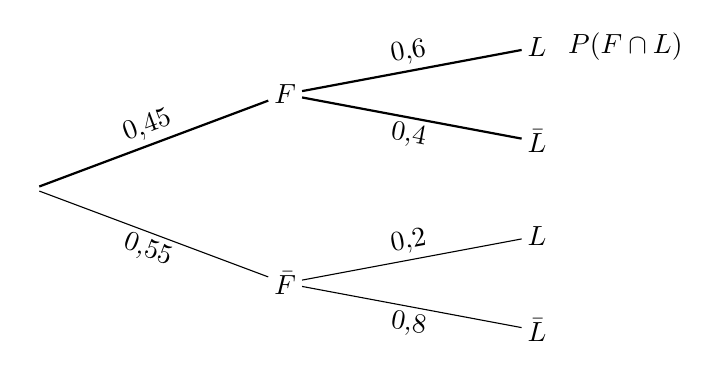
\begin{tikzpicture}[
				grow=right,
				level 1/.style={level distance=3.2cm, sibling distance=2.4cm},
				level 2/.style={level distance=3.2cm, sibling distance=1.2cm},
				every node/.style={inner sep=2pt}
			]
			\node {}
			child { node { $\bar{F}$ }
					child { node { $\bar{L}$ } edge from parent node[sloped, below] { $0{,}8$ } }
					child { node { $L$ } edge from parent node[sloped, above] { $0{,}2$ } }
					edge from parent node[sloped, below] { $0{,}55$ }
				}
			child { node { $F$ }
					child { node { $\bar{L}$ } edge from parent node[sloped, below] { $0{,}4$ } }
					child { node { $L$ }
							node[right=0.2cm] {$\rarr\ P(F \cap L)$}
							edge from parent[thick] node[sloped, above] { $0{,}6$ }
						}
					edge from parent[thick] node[sloped, above] { $0{,}45$ }
				};
		\end{tikzpicture}
	\end{center}

	\begin{enumerate}
		\item \textbf{Justification des valeurs manquantes (règle des n\oe{}uds) :}
		      \begin{itemize}
			      \item S'il y a $45\%$ de filles dans le lycée, alors le reste de la population est constitué de garçons, soit $55\%$.
			            \[
				            P(\bar{F}) = 1 - 0{,}45 = 0{,}55
			            \]
			      \item Si $60\%$ des filles ont les cheveux longs, alors les $40\%$ de filles restantes ont les cheveux courts :
			            \[
				            P_F(\bar{L}) = 1 - 0{,}6 = 0{,}4
			            \]
		      \end{itemize}

		\item \textbf{Calcul de la probabilité d'une intersection :}
		      Pour calculer la probabilité de choisir une fille aux cheveux longs, on multiplie les probabilités rencontrées le long du chemin passant par $F$ puis par $L$ :
		      \[
			      P(F \cap L) = P(F) \times P_F(L) = 0{,}45 \times 0{,}6 = 0{,}27
		      \]
		      Il y a donc $27\%$ de chances de choisir une fille aux cheveux longs dans ce lycée.
	\end{enumerate}
\end{ex}

\subsection{Formule des probabilités totales}

\begin{thm}[Formule des probabilités totales]
	Soit $A$ un événement et $\bar{A}$ son événement contraire. Pour tout événement $B$, sa probabilité est donnée par la somme des probabilités des chemins menant à $B$ :
	\[
		P(B) = P(A \cap B) + P(\bar{A} \cap B)
	\]

	Soit sous forme développée :
	\[
		P(B) = P(A) \times P_A(B) + P(\bar{A}) \times P_{\bar{A}}(B)
	\]

	\begin{center}
		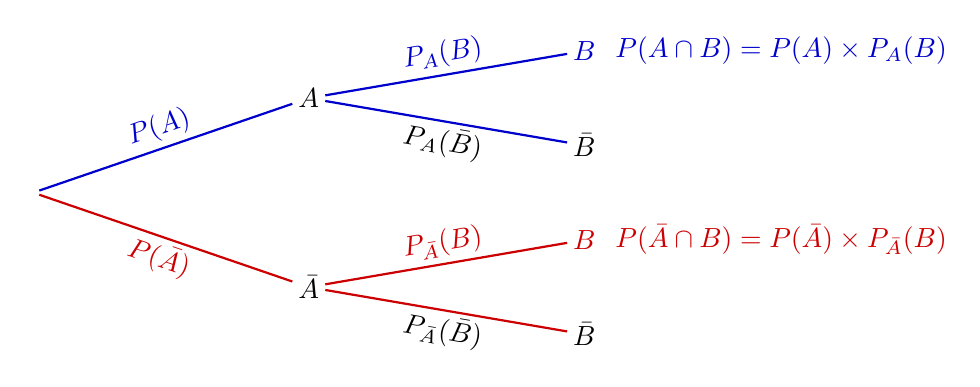
\begin{tikzpicture}[
				grow=right,
				level 1/.style={level distance=3.5cm, sibling distance=2.4cm},
				level 2/.style={level distance=3.5cm, sibling distance=1.2cm},
				every node/.style={inner sep=2pt}
			]
			\node {}
			child { node { $\bar{A}$ }
					child { node { $\bar{B}$ }
							edge from parent node[sloped, below] { $P_{\bar{A}}(\bar{B})$ }
						}
					child { node[red!80!black] { $B$ }
							node[right=0.2cm, red!80!black] {$\rarr\  P(\bar{A} \cap B) = P(\bar{A}) \times P_{\bar{A}}(B)$}
							edge from parent[red!80!black, thick] node[sloped, above] { $P_{\bar{A}}(B)$ }
						}
					edge from parent[red!80!black, thick] node[sloped, below] { $P(\bar{A})$ }
				}
			child { node { $A$ }
					child { node { $\bar{B}$ }
							edge from parent node[sloped, below] { $P_A(\bar{B})$ }
						}
					child { node[blue!80!black] { $B$ }
							node[right=0.2cm, blue!80!black] {$\rarr\  P(A \cap B) = P(A) \times P_A(B)$}
							edge from parent[blue!80!black, thick] node[sloped, above] { $P_A(B)$ }
						}
					edge from parent[blue!80!black, thick] node[sloped, above] { $P(A)$ }
				};
		\end{tikzpicture}
	\end{center}
\end{thm}

\newpage

\begin{methode}[Appliquer la formule des probabilités totales]
	Une maladie touche $2\%$ d'une population. Un test de dépistage donne les résultats suivants :
	\begin{itemize}
		\item Si un individu est malade $\pa{M}$, le test est positif $\pa{T}$ dans $85\%$ des cas.
		\item Si un individu est sain $\pa{\bar{M}}$, le test est négatif $\pa{\bar{T}}$ dans $95\%$ des cas.
	\end{itemize}

	\textbf{1. Modélisation par un arbre pondéré :}

	\begin{center}
		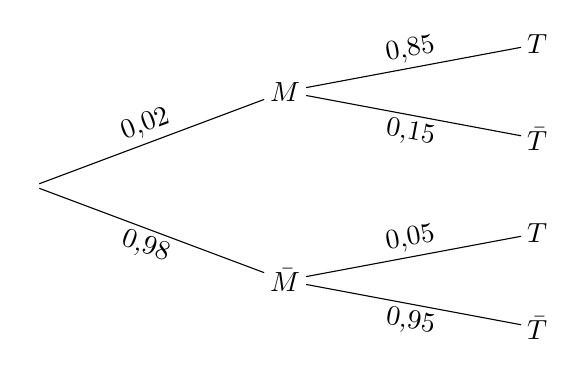
\begin{tikzpicture}[
				grow=right,
				level 1/.style={level distance=3.2cm, sibling distance=2.4cm},
				level 2/.style={level distance=3.2cm, sibling distance=1.2cm},
				every node/.style={inner sep=2pt}
			]
			\node {}
			child { node { $\bar{M}$ }
					child { node { $\bar{T}$ } edge from parent node[sloped, below] { $0{,}95$ } }
					child { node { $T$ } edge from parent node[sloped, above] { $0{,}05$ } }
					edge from parent node[sloped, below] { $0{,}98$ }
				}
			child { node { $M$ }
					child { node { $\bar{T}$ } edge from parent node[sloped, below] { $0{,}15$ } }
					child { node { $T$ } edge from parent node[sloped, above] { $0{,}85$ } }
					edge from parent node[sloped, above] { $0{,}02$ }
				};
		\end{tikzpicture}
	\end{center}

	\textbf{2. Calcul de la probabilité que le test soit positif $P(T)$ :}

	D'après la formule des probabilités totales :
	\[
		\begin{array}{rccccl}
			P(T) & = & P(M \cap T)        & + & P(\bar{M} \cap T)                &                         \\
			     & = & P(M) \times P_M(T) & + & P(\bar{M}) \times P_{\bar{M}}(T) &                         \\
			     & = & 0,02 \times 0,85   & + & 0,98 \times 0,05                 & = 0,017 + 0,049 = 0,066
		\end{array}
	\]

	La probabilité d'avoir un test positif est égale à $0,066$ (soit $6,6\%$).

	Dans les applications médicales, les probabilités conditionnelles liées à un test de dépistage portent des noms particuliers :

	\begin{itemize}
		\item \textbf{La sensibilité :} C'est la probabilité que le test soit positif sachant que l'individu est malade, soit :
		      \[
			      P_M(T) = 0{,}85
		      \]

		      Elle mesure la capacité du test à détecter la maladie.
		\item \textbf{La spécificité :} C'est la probabilité que le test soit négatif sachant que l'individu est sain, soit :
		      \[
				  P_{\bar{M}}\pa{\bar{T}} = 0{,}95
		      \]

		      Elle mesure la capacité du test à cibler uniquement les personnes malades.
	\end{itemize}
\end{methode}


